%!TEX program = xelatex
% Note: this template must be compiled with XeLaTeX rather than PDFLaTeX
% due to the custom fonts used. The line above should ensure this happens
% automatically, but if it doesn't, your LaTeX editor should have a simple toggle
% to switch to using XeLaTeX.

\documentclass[
  aspectratio=169, % Uncomment to use an aspect ratio of 16:9 (160 mm by 90 mm)
  %aspectratio=43, % Uncomment to use an aspect ratio of 4:3 (128mm by 96mm)
  t, % Top align all slide content by default
  onlytextwidth, % Typeset content in columns at text width
  10pt, % Default font size, use 10pt for the 16:9 aspect ratio and 8pt for the 4:3 aspect ratio
]{beamer}

\usepackage{../ImperialTheme/beamerthemeImperial} % Use the Imperial theme

\def\imagefolder{../ImperialTheme/Images/}
\def\Rey{\text{Re}}
\title{Transient growth in flat plate} % Presentation title to appear on the title slide and left footers

\subtitle{} % Presentation subtitle to appear on the title slide

\author{Víctor Ballester} % Author name(s) to appear on the title slide

\date{\today} % Presentation date to appear on the title slide and right footers

\begin{document}

\begingroup
\setbeamercolor{background canvas}{bg=ICLBlue} % Slide background color
\setbeamercolor{title page title}{fg=white} % Title text color
\setbeamercolor{title page subtitle}{fg=white} % Subtitle text color
\setbeamercolor{author}{fg=white} % Author(s) text color
\setbeamercolor{date}{fg=white} % Date text color
\setbeamertemplate{title page}[logo]{\imagefolder/ICL_Logo_White.pdf} % Imperial logo color, use 'ICL_Logo_White.pdf' for white and 'ICL_Logo_Blue.pdf' for blue
\frame[plain, s]{\titlepage} % Output the title page with no footer ('plain') and vertically distributed text ('s')
\endgroup

\begin{frame}
	\frametitle{Transient growth in flat plate}
	\begin{itemize}
		\item I tried transient growth in the flat plate.
		\item The length of the domain is $1000 (\text{downstream}) - (-100 \text{upstream}) = 1100$, as if it was a $0-$width gap domain. So I tried transient growth with $\tau = 450, 900$, $\tau$ being the time the simulation is evolved forwards and then backwards. It turned out that the phase speed of the TS modes is not 1 (of course, I didn't thought about that), it is much less (I estimated it to be around $0.35$), so I get and amplification just until half of the domain more or less. Even though, \textbf{should I increase the length of the domain?}
		\item Now I am running the case for larger $\tau$.
	\end{itemize}
	\centering
	
\includegraphics[width=0.85\linewidth]{Images/ts_tg.png}
\end{frame}
\begin{frame}
	\centering
	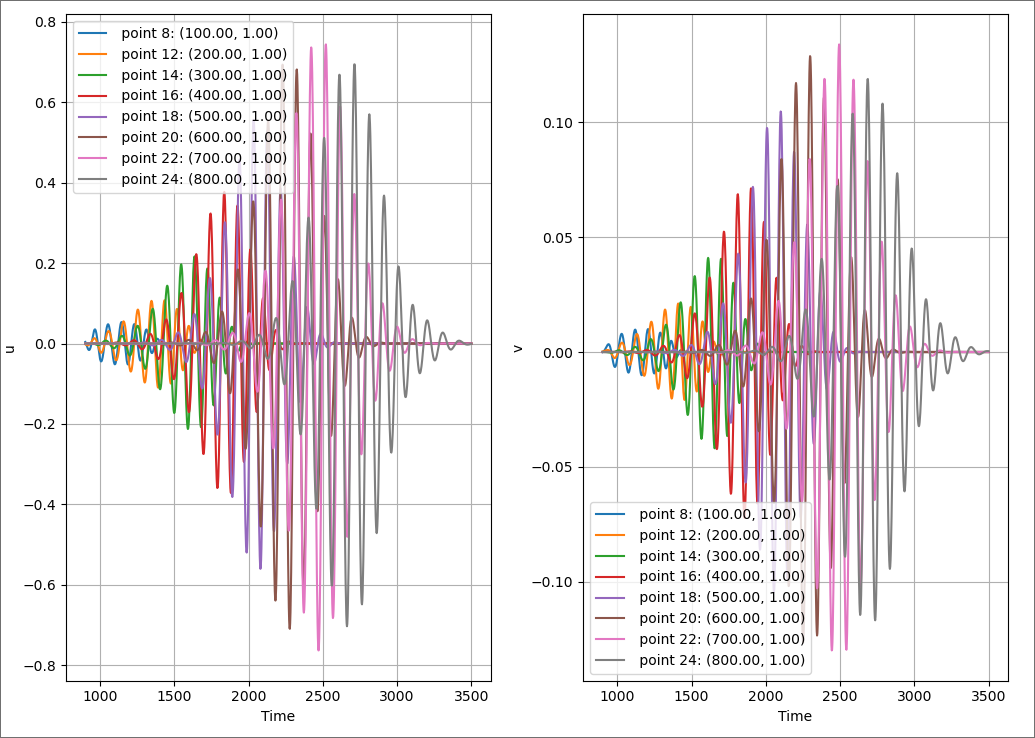
\includegraphics[width=0.75\linewidth]{Images/ts_tg_plot.png}
\end{frame}
\begin{frame}
	\frametitle{Harmonic analysis of the orange-to-red change}
	\centering
	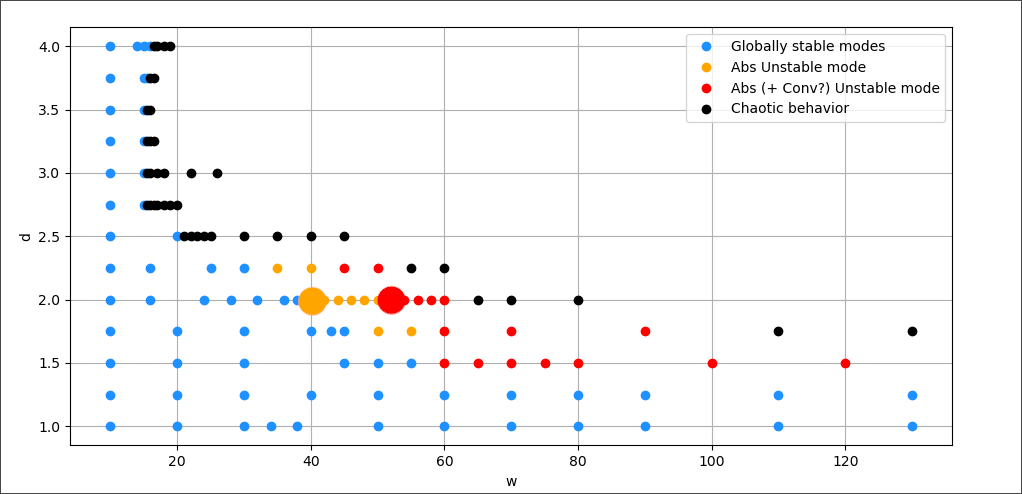
\includegraphics[width=0.75\linewidth]{Images/stability_curve.png}
	% \begin{itemize}
	% 	\item I realized I input the wrong frequency when blowing and suction, up to a factor of 1.72. Now I am redoing the computations. Could that explain that all the curves where clustered together?
	% 	\item I also try global stability analysis with the coupled approach, which worked (so far with low polynomial order), but it only does $kdim$ iterations and $kdim$ is bounded by 500 in the code. Why?
	% \end{itemize}
	% \centering
	% 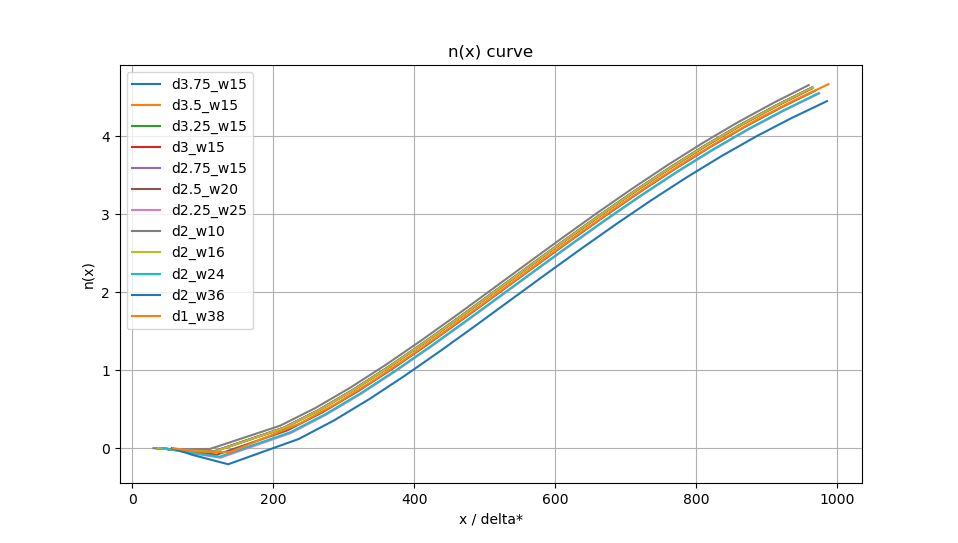
\includegraphics[width=0.5\linewidth]{Images/nfactorCurve.png}
\end{frame}
\begin{frame}
	\centering
	\begin{columns}[T] % [T] ensures correct vertical alignment
		\begin{column}{0.48\linewidth} % Left column
			\textcolor{orange}{\textbf{$d=2, w=40$}}

			Freq with highest amplitude for u
			$ \omega : 0.00000000, Amplitude: 226.23665390$
			$ \omega : 0.16174536, Amplitude: 0.33523849$
			$ \omega : 0.23173134, Amplitude: 0.25998462$
			$ \omega : 0.23328658, Amplitude: 5.02840019$
			$ \omega : 0.23484183, Amplitude: 0.28651745$

			Freq with highest amplitude for v
			$ \omega : 0.00000000, Amplitude: 1.77348566$
			$ \omega : 0.16174536, Amplitude: 0.40399285$
			$ \omega : 0.23173134, Amplitude: 0.33448704$
			$ \omega : 0.23328658, Amplitude: 6.55379325$
			$ \omega : 0.23484183, Amplitude: 0.37806377$
			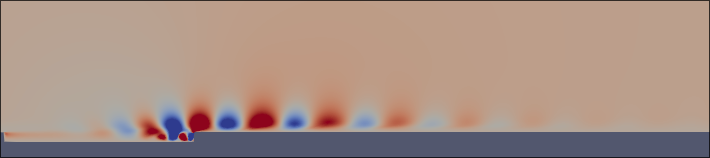
\includegraphics[width=\linewidth]{Images/d2_w40.png}
		\end{column}
		\begin{column}{0.48\linewidth} % Left column
			\textcolor{red}{\textbf{$d=2, w=52$}}

			Freq with highest amplitude for u
			$ \omega : 0.00000000, Amplitude: 48.38968907$
			$ \omega : 0.02559816, Amplitude: 3.03884201$
			$ \omega : 0.06050475, Amplitude: 2.12776977$
			$ \omega : 0.08610291, Amplitude: 2.39670993$
			$ \omega : 0.08843002, Amplitude: 1.72555528$

			Freq with highest amplitude for v
			$ \omega : 0.02559816, Amplitude: 3.28989416$
			$ \omega : 0.06050475, Amplitude: 1.56887596$
			$ \omega : 0.08610291, Amplitude: 2.97408531$
			$ \omega : 0.08843002, Amplitude: 2.26994456$
			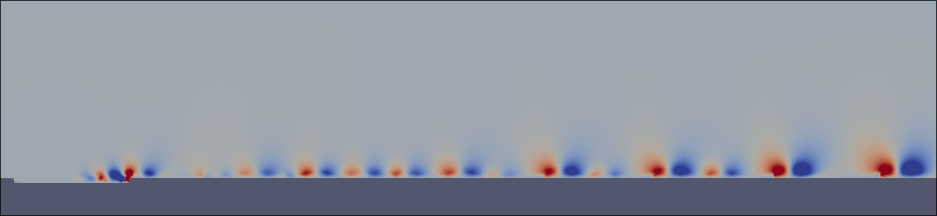
\includegraphics[width=\linewidth]{Images/d2_w52.png}
		\end{column}
	\end{columns}
	\centering
\end{frame}
\begin{frame}
  \frametitle{Neutral curve blasius}
  \begin{itemize}
    \item Inside the curve, convectively unstable; outside, convectively stable.
  \end{itemize}
  
  \centering
	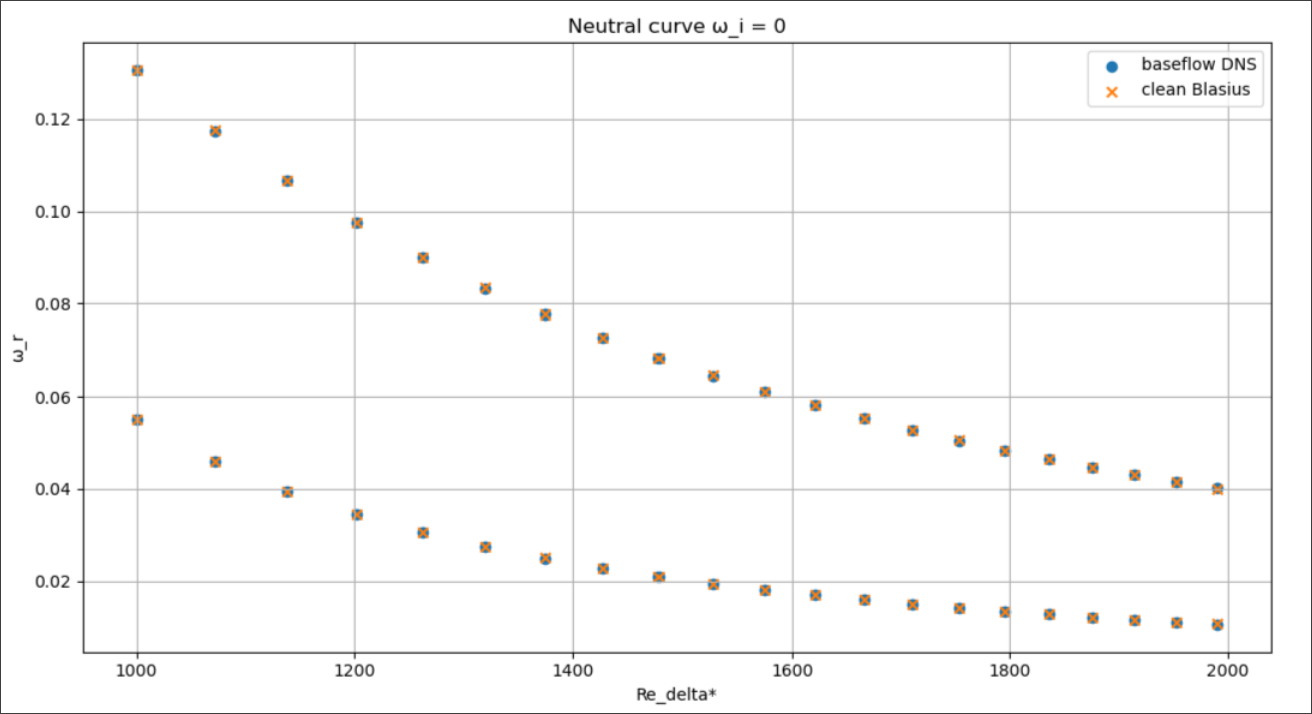
\includegraphics[width=0.75\linewidth]{Images/neutralcurve.png}
\end{frame}
\end{document}
